\begin{center}
\Large
\textbf{Площади. 07 июля.  }
\end{center}


\noindent{\sc Определение.} Каждой фигуре $M$ на плоскости ставится в соответствие
число $S_M$, называемое {\it площадью}, такое, что выполнены следующие
свойства:

1)~$S_M\geq 0$;

2)~Площади равных фигур равны;

3)~Если фигура $M$ состоит из фигур $A$ и $B$, не имеющих общих внутренних
точек, то $S_M = S_A + S_B$;

4)~Площадь квадрата со стороной  $x$ равна $x^2$.


\begin{enumerate}

\item Из того, что площадь квадрата со стороной $x$ равна $x^{2}$ выведите, что площадь прямоугольника со сторонами $a$ и $b$ равна $ab$.

\item а)~Докажите, что площадь прямоугольного треугольника равна половине произведения
его катетов.\\
б)~Докажите, что площадь остроугольного треугольника равна половине произведения
произвольной его стороны на опущенную на эту сторону высоту.\\
в)~Докажите то же самое утверждение для произвольного треугольника.\\
г)~Докажите, что площадь параллелограмма равна произведению
произвольной его стороны на опущенную на эту сторону высоту.\\
д)~Докажите, что площадь трапеции равна произведению полусуммы оснований на высоту.

\item 
Диагонали трапеции $ABCD$ с основаниями $AD$ и~$BC$ пересекаются в точке $O$.
Докажите, что $S_{AOB} = S_{COD}$.

\item а) Докажите, что медиана делит треугольник на два равновеликих.\\
б) Докажите, что медианы треугольника пересекаются в одной точке, делятся точкой пересечения в отношении $2 : 1$, считая от вершины,
и делят треугольник на 6 равновеликих.


\item Каждую сторону треугольника площади $S$ продлили на её длину (см. рисунок). Чему равна площадь большого треугольника?
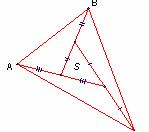
\includegraphics[width=0.2\textwidth]
{square.JPG}

\item Дан выпуклый четырехугольник $ABCD$. На лучах $AB$, $BC$, $CD$ и $DA$ выбраны такие точки $A_1$, $B_1$, $C_1$ и $В_1$, что $AB=A_1B$, $BC=B_1C$, $CD=C_1D$ и $DA=D_1A$. Найдите отношение $S(A_1B_1C_1D_1)/S(ABCD)$.


\item Дан треугольник $ABC$. На луче~$BC$ взята точка~$C_1$.\\
а)~Докажите, что $\frac{S_{ABC_1}}{S_{ABC}} = \frac{|BC_1|}{|BC|}$.\\
б)~Пусть, кроме того, на луче~$BA$ взята точка~$A_1$. Докажите, что
$\frac{S_{A_1BC_1}}{S_{ABC}} = \frac{|BA_1|\cdot |BC_1| }{|BA| \cdot |BC|}$

{\it Вывод: площади треугольников с общим углом относятся, как произведения сторон, этот угол заключающих}

в)~Докажите, что это верно и в случае, когда углы не равны, а дополняют
друг друга до~$180^\circ$.



\item В треугольнике $ABC$ проведена биссектриса $BL$. Докажите, что $\frac{|AL|}{|CL|}=\frac{|AB|}{|CB|}$.

\item а)~Две параллельные прямые пересекают стороны угла с вершиной~$O$ в точках
$A$, $B$ и $A_1$, $B_1$ соответственно. Докажите, что~$\frac{|OA|}{|OB|} = \frac {|OA_1|}{|OB_1|}$.\\
б)~({\bf Теорема Фалеса}) Три параллельные прямые пересекают стороны угла с вершиной~$O$ в точках
$A$, $B$, $C$ и $A_1$, $B_1$, $C_1$ соответственно. Докажите, что~$\frac{|AB|}{|BC|} = \frac {|A_1B_1|}{|B_1C_1|}$.\\
в) ({\bf Обратная теорема Фалеса}) Две прямые пересекли стороны угла с вершиной $O$ в точках $A_{1},B_{1}$ и $A_{2}, B_{2}$ соответственно. Оказалось, что $\frac{|OA|}{|OB|} = \frac {|OA_1|}{|OB_1|}$. Докажите, что эти прямые параллельны.


\end{enumerate}